\chapter{BPSK Waveform Generation}

\section{Input Bit Sequence}
For waveform visualization, the assigned 10-bit sequence is
\[
1,\,0,\,1,\,1,\,0,\,0,\,1,\,0,\,1,\,0
\]

This sequence is used to generate the complete transmitted BPSK waveform by concatenating the one-bit BPSK symbols.

\section{Python Implementation}
The following Python code generates the 10-bit BPSK waveform and marks the bit boundaries on the plot.

\begin{lstlisting}[style=pythonstyle, caption={10-Bit BPSK Waveform Generation}]
import numpy as np
import matplotlib.pyplot as plt

A = 1
fc = 15000
Rb = 1000
fs = 200000

Tb = 1 / Rb
N = int(fs / Rb)
t_bit = np.arange(0, Tb, 1/fs)

s1 = A * np.cos(2 * np.pi * fc * t_bit)
s0 = -A * np.cos(2 * np.pi * fc * t_bit)

bits = np.array([1,0,1,1,0,0,1,0,1,0])
waveform = np.array([])

for bit in bits:
    if bit == 1:
        waveform = np.concatenate((waveform, s1))
    else:
        waveform = np.concatenate((waveform, s0))

timeaxis = np.arange(len(waveform)) / fs

plt.figure(figsize=(12,4))
plt.plot(timeaxis, waveform, linewidth=1.2)
for k in range(len(bits) + 1):
    plt.axvline(k * Tb, color='red', linestyle='--', linewidth=0.8)

plt.xlabel('Time (s)')
plt.ylabel('Amplitude (V)')
plt.title('10-Bit BPSK Waveform')
plt.grid(True)
plt.tight_layout()
plt.show()
\end{lstlisting}

\section{Results and Discussion}
The generated waveform shows how binary data is carried using phase changes of the same cosine carrier. A bit value of 1 is represented by a cosine wave, while a bit value of 0 is represented by the same wave with 180-degree phase reversal.

The vertical dashed lines indicate bit boundaries, so it becomes easy to see where each bit starts and ends. Whenever the bit changes from 1 to 0 or 0 to 1, the waveform flips its phase, which is the main visual signature of BPSK.

\begin{figure}[htbp]
    \centering
    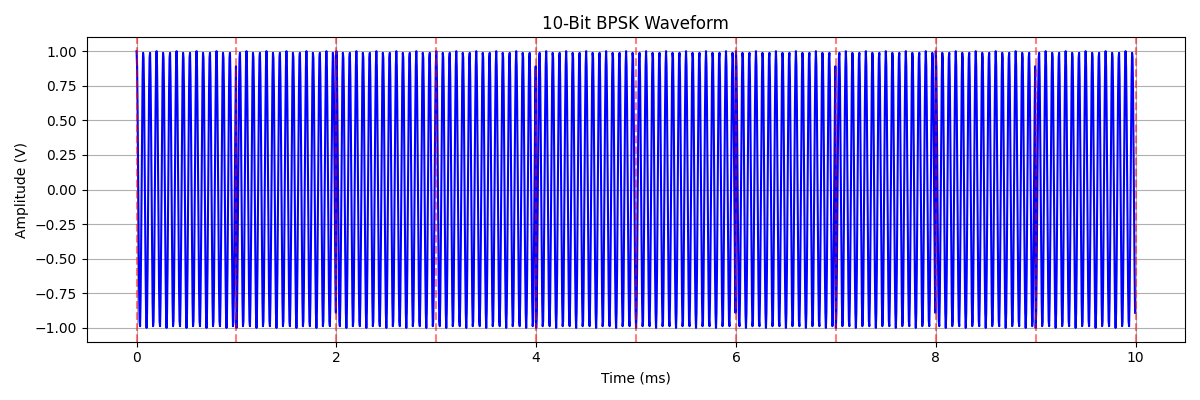
\includegraphics[width=0.8\textwidth]{plots/10-bit_wave.png}
    \caption{10-bit BPSK waveform with bit boundaries}
\end{figure}